\documentclass[a4paper,10pt]{article}
\usepackage{fontspec}
\setmainfont[Path=fonts/,BoldFont=FandolSong-Bold.otf,ItalicFont=FandolSong-Regular.otf]{FandolSong-Regular.otf}
\XeTeXlinebreaklocale "zh"
\XeTeXlinebreakskip=0pt plus 1pt
\usepackage[left=24mm,right=24mm,top=22mm,bottom=22mm]{geometry}
\usepackage{graphicx,float,booktabs,array,caption,titlesec,fancyhdr,indentfirst}
\usepackage[hidelinks,unicode]{hyperref}
\hypersetup{pdfauthor={},pdftitle={公开口碑信息对餐饮商户经营风险画像的验证},pdfsubject={赛题三，队名待填写的报告稿}}
\renewcommand{\normalsize}{\fontsize{10.5bp}{15.75bp}\selectfont}
\normalsize
\setlength{\parindent}{21bp}
\setlength{\parskip}{0pt}
\setlength{\tabcolsep}{4pt}
\newlength{\tablewidth}
\renewcommand{\arraystretch}{1.05}
\setlength{\textfloatsep}{6pt}
\setlength{\intextsep}{6pt}
\captionsetup{labelformat=empty,font=normalsize,skip=3pt}
\titleformat{\section}{\normalfont\fontsize{12pt}{18pt}\selectfont\bfseries}{}{0pt}{}
\titlespacing*{\section}{0pt}{6pt}{4pt}
\pagestyle{fancy}
\fancyhf{}
\fancyfoot[C]{\fontsize{9pt}{12pt}\selectfont\thepage}
\renewcommand{\headrulewidth}{0pt}
\setlength{\headheight}{0pt}
\setlength{\footskip}{12mm}
\emergencystretch=1em
\begin{document}
\begin{titlepage}
\centering
\vspace*{30mm}
{\fontsize{15pt}{23pt}\selectfont 2026 FinTechathon 深圳国际金融科技大赛\par}
\vspace{5mm}
{\fontsize{12pt}{18pt}\selectfont 数据分析赛道 · 赛题三\par}
\vspace{26mm}
{\fontsize{20pt}{30pt}\selectfont\bfseries 从公开口碑到复核决策：餐饮商户经营风险指标构建与验证\par}
\vspace{5mm}
{\fontsize{13pt}{21pt}\selectfont ——可解释画像、预算验证与日期偏差审计\par}
\vspace{30mm}
{\fontsize{14pt}{21pt}\selectfont 小组名称：待填写\par}
\end{titlepage}
\setcounter{page}{1}
\normalsize
\section*{摘要}
针对小微餐饮主体财务信息稀缺的问题，本文研究公开口碑信息能否补充经营风险画像。基于某生活服务平台的海外历史区域子集，筛选674家餐饮商户，其中123家记录为停止营业；围绕口碑质量、评论活跃度和低分评论主题构建12项指标，比较逻辑回归与梯度提升树的六种输入组合，并进行独立测试和人工复核预算模拟。按验证集确定的增强逻辑回归，测试ROC-AUC为0.577、平均精确率AP为0.220；相对评分质量基线的AP增量为0.009，95\%配对Bootstrap区间包含0。预设增强树模型AP为0.319，在复核14家测试商户时命中7家停止营业商户，相对随机名单的点估计提升2.70倍，但区间仍包含无提升的可能。补充同年份配对审计后，增强树模型AUC由0.631降至0.488，提示总体优势可能受年代结构影响。本文形成“画像—复核—反馈”的产品闭环与收益检验条件；结果支持调查线索构建，尚未证明前瞻经营或信用风险识别增益。

关键词：公开数据；餐饮商户；经营风险画像；营业状态；人工复核

\section*{一、业务背景与研究问题}
小微经营主体现金流缓冲有限，传统财务风控又依赖标准化报表和信用记录。生活服务平台的公开评价覆盖消费体验、商户活跃度及经营环境，为信息稀疏主体提供了另一条观察路径。但公开评分与经营风险的关系可能受到平台选择、商户规模和时间结构影响，必须用独立样本验证，不能把低评分直接等同于高信用风险。

研究依次回答“信息能否量化、量化是否有效、有效是否值得使用”：构建口碑、活跃度及主题指标；相对评分基线检验增量；在固定核查预算下验证排序价值。贡献在于将指标构建、保留测试、预算验证和日期偏差审计串联，形成可复验的决策证据链。研究以餐饮商户为代理，以公开营业状态作替代验证标签。

赛题强调在经营流水基础上引入公开信息。本研究未获得真实流水，因此检验的是公开信息的独立识别价值，尚未验证其对流水模型的增益。样本也缺少企业规模和贷款表现，餐饮商户仅作为小微主体的研究代理。停业可能来自搬迁或主动退出等原因，不等于财务困境。


\newpage
\section*{二、数据介绍与样本清洗}
原始来源为某生活服务平台的学术开放数据[1]，实际使用其社区发布的区域子集[2]。子集以城市名称包含“leveland”的规则筛选，覆盖Cleveland及邻近区域。本研究固定数据来源提交并校验两个输入文件，独立计算指标和模型，没有复用来源项目的模型结果。商户表含类别、城市和营业状态；评论表含商户ID、日期、评分和文本。

原始数据含3,164家商户、91,057条评论。评论日期为2005年4月15日至2017年7月26日，营业状态的采集日期未说明。1,361家餐饮商户中，318家标记停止营业；其评论共64,693条。按照评价数量、历史跨度及近期可观测性逐步筛选，最终纳入674家，其中营业551家、停止营业123家，停止营业占比18.25\%。

\begin{figure}[H]
\centering
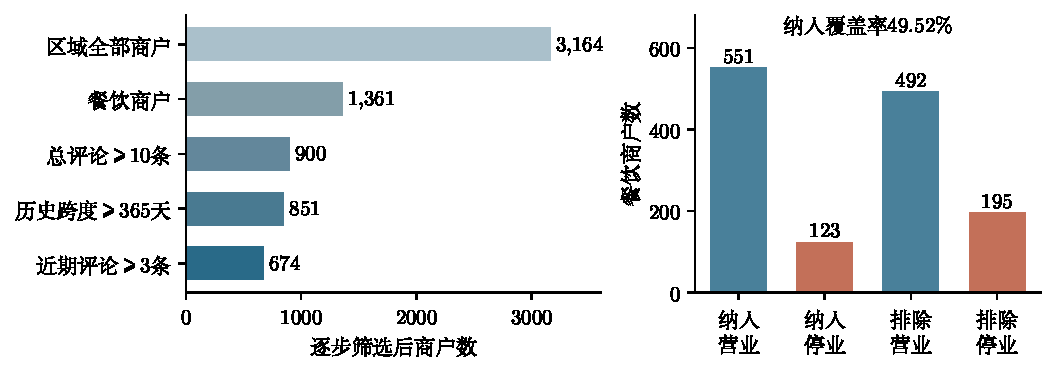
\includegraphics[width=1\linewidth]{figures/figure01_sample.pdf}
\caption{图1 样本逐步筛选及最终营业状态分布}
\end{figure}
\begin{table}[H]
\centering
\caption{表1 数据质量与样本纳入规则}
\setlength{\tablewidth}{\linewidth}
\addtolength{\tablewidth}{-4\tabcolsep}
\begin{tabular}{>{\raggedright\arraybackslash}p{0.270\tablewidth}>{\raggedright\arraybackslash}p{0.730\tablewidth}}
\toprule
\textbf{核对项目} & \textbf{结果或处理规则} \\
\midrule
商户与评论关联 & 商户ID无重复；评论ID无重复；评论均匹配商户 \\
日期与评分 & 无无效日期；评分均处于1—5分 \\
纳入门槛 & 总评论≥10条；历史跨度≥365天；近180天评论≥3条 \\
计数一致性 & 64家商户表总评论数与实际评论数不一致，原因未确认 \\
计数处理 & 所有计数从实际评论重新计算，不使用商户表总数 \\
\bottomrule
\end{tabular}
\end{table}
最终样本包含核心城区商户635家、邻近城区39家。筛选排除了新店、评价较少及长期无评论的商户，改善指标可观测性，也形成样本选择偏差。全部报告图表均为匿名聚合结果，不展示商户名称、评论者信息或原始评论。


\newpage
\section*{三、指标体系与描述性分析}
以各商户最后一条评论日期作为历史窗口锚点：近360天为距锚点0—359天，近期与前期分别为0—179天和180—359天。窗口在不同商户之间不对应统一日历时间，因而本设计属于历史横截面比较。基于经营机制构建三类、共12项指标，见表2。

\begin{table}[H]
\centering
\caption{表2 三维经营风险画像指标体系}
\setlength{\tablewidth}{\linewidth}
\addtolength{\tablewidth}{-6\tabcolsep}
\begin{tabular}{>{\raggedright\arraybackslash}p{0.180\tablewidth}>{\raggedright\arraybackslash}p{0.480\tablewidth}>{\raggedright\arraybackslash}p{0.340\tablewidth}}
\toprule
\textbf{维度} & \textbf{指标（每维4项）} & \textbf{业务含义} \\
\midrule
口碑质量Q & 近360天均分、低分占比、评分标准差；近期较前期均分变化 & 衡量消费者评价水平、分歧及变化 \\
评论活跃度A & 近期/前期评论数；数量对数变化；六个30天窗口数量变异系数 & 衡量平台消费关注度及波动 \\
低分主题T & 近期低分且提及服务、卫生、价格、食物问题的评论占比 & 识别可供调查核实的经营体验线索 \\
\bottomrule
\end{tabular}
\end{table}
数量变化定义为log(1+近期数量)-log(1+前期数量)。低分指评分不超过2分；各主题以固定词典匹配，分母为近期全部评论数。40家商户前期窗口无评论，其均分变化记为缺失，在拟合数据上作中位数填补并增加缺失指示。评论数不是客流或营业额，词典主题也未经独立人工标注验证。

\begin{figure}[H]
\centering
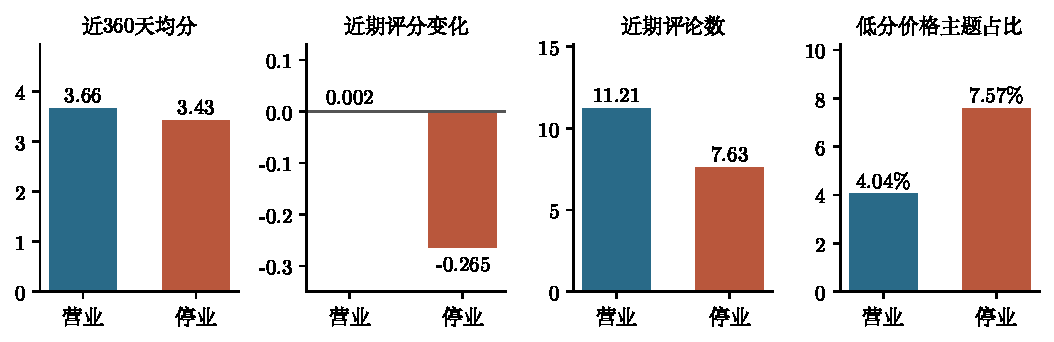
\includegraphics[width=1\linewidth]{figures/figure02_descriptive.pdf}
\caption{图2 营业与停止营业商户的主要指标均值（全样本探索性描述）}
\end{figure}
停止营业商户近360天均分为3.43，营业商户为3.66；近期评分变化均值分别为-0.265与0.002。近期评论数均值分别为7.63与11.21，但两组中位数均为7，说明分布偏态。12项Mann–Whitney检验作Holm校正后，仅均分和价格主题在0.05水平有差异（校正p=0.0065、0.0487）；评分变化p=0.0538，卫生主题未呈预期方向。描述差异不等于独立预测价值，主题提及也不代表因果关系。


\newpage
\section*{四、模型分析与验证设计}
以商户表记录的停止营业为正类，营业为负类。按商户独立、标签分层，一次固定划分训练、验证、测试集合，随机种子为20261011。同一商户不会跨集合，测试集保留到参数与主分析方案确定后使用；划分比例为60\%/20\%/20\%，见表3。

\begin{table}[H]
\centering
\caption{表3 样本划分与标签构成}
\setlength{\tablewidth}{\linewidth}
\addtolength{\tablewidth}{-8\tabcolsep}
\begin{tabular}{>{\raggedright\arraybackslash}p{0.310\tablewidth}>{\raggedright\arraybackslash}p{0.230\tablewidth}>{\raggedright\arraybackslash}p{0.230\tablewidth}>{\raggedright\arraybackslash}p{0.230\tablewidth}}
\toprule
\textbf{集合} & \textbf{商户数} & \textbf{停止营业数} & \textbf{占比} \\
\midrule
训练集 & 404 & 73 & 18.07\% \\
验证集 & 135 & 25 & 18.52\% \\
测试集 & 135 & 25 & 18.52\% \\
\bottomrule
\end{tabular}
\end{table}
采用逻辑回归（LR）作解释性基线，以及直方图梯度提升树（HGB）检验非线性关系。每种算法均比较Q、Q+A、Q+A+T三组输入，共六个预设模型，以分离评分、活跃度与评论主题的增量。没有将当前营业状态文字、关闭词汇、最后评论年份或距数据末日的无评论天数放入模型。

逻辑回归在C=0.1、1、10中选择正则强度；树模型比较最大叶节点7、15及L2系数1、5，固定150次迭代、学习率0.05、每叶最少20个样本。每种算法与指标组仅用验证集平均精确率AP选参数，再合并训练和验证集重新拟合。逻辑回归标准化、所有缺失填补及缺失指示均只在拟合数据估计。

质量基线在LR·Q与HGB·Q中按验证集AP选择，增强方案在LR·QAT与HGB·QAT中同样选择。由此主分析基线为LR·Q，主分析增强模型为LR·QAT。增强树模型虽然测试表现较好，但没有据此回头改选为主模型。全部预设模型均保留，并明确区分主分析与探索比较。

验证使用ROC-AUC、平均精确率AP和有限预算下的复核命中率、捕获率及提升倍数。AP采用非插值平均精确率，不混用梯形积分PR面积；测试停止营业比例18.52\%作为随机排序AP的总体参考。对测试商户作1,500次配对Bootstrap，报告百分位95\%区间；该区间不涵盖训练重拟合、模型选择或外部地区的不确定性。


\newpage
\section*{五、模型结果与增量价值}
六个模型的独立测试点估计和Bootstrap区间见图3。质量基线LR·Q测试ROC-AUC为0.545、AP为0.211；主分析增强LR·QAT分别为0.577和0.220。加入活跃度与主题后的改善较小，不能据此声称公开信息已显著提升风险识别。

\begin{figure}[H]
\centering
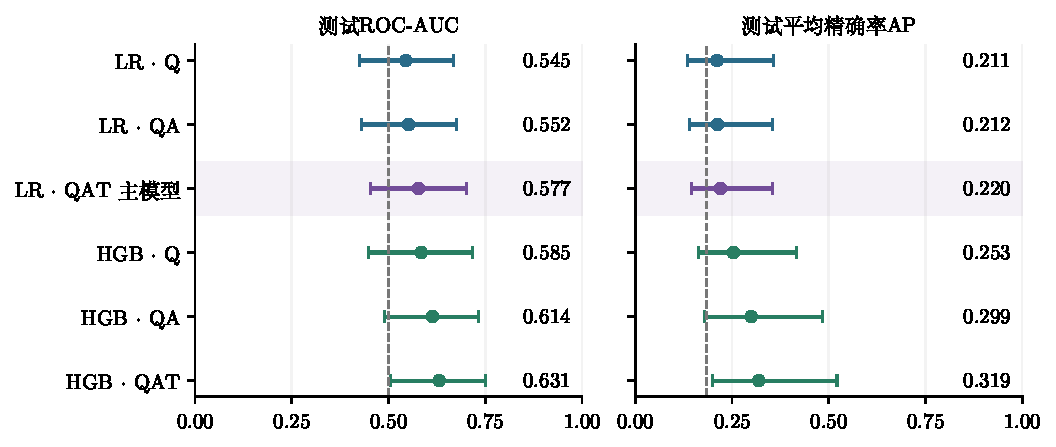
\includegraphics[width=1\linewidth]{figures/figure03_models.pdf}
\caption{图3 六个预设模型的测试表现及95\%Bootstrap区间；虚线为随机参考}
\end{figure}
\begin{table}[H]
\centering
\caption{表4 预设模型的验证与测试结果}
\setlength{\tablewidth}{\linewidth}
\addtolength{\tablewidth}{-8\tabcolsep}
\begin{tabular}{>{\raggedright\arraybackslash}p{0.370\tablewidth}>{\raggedright\arraybackslash}p{0.190\tablewidth}>{\raggedright\arraybackslash}p{0.240\tablewidth}>{\raggedright\arraybackslash}p{0.200\tablewidth}}
\toprule
\textbf{模型} & \textbf{验证AP} & \textbf{测试ROC-AUC} & \textbf{测试AP} \\
\midrule
LR·Q & 0.301 & 0.545 & 0.211 \\
LR·QA & 0.320 & 0.552 & 0.212 \\
LR·QAT（主模型） & 0.344 & 0.577 & 0.220 \\
HGB·Q & 0.259 & 0.585 & 0.253 \\
HGB·QA & 0.323 & 0.614 & 0.299 \\
HGB·QAT & 0.304 & 0.631 & 0.319 \\
\bottomrule
\end{tabular}
\end{table}
主模型相对质量基线的AP增量为0.0091，配对95\%区间为[-0.055，0.064]。增强树模型相对其质量基线的AP增量为0.0658，区间为[-0.038，0.185]。两者均包含0，无法排除无增益的情况。树模型中QA相对Q、QAT相对QA的AP点估计均有所增加，可作为扩大样本后进一步验证的线索。

本次测试仅含25家停止营业商户，区间较宽；多模型比较未作家族显著性校正，结果应按探索性证据理解。模型输出仅表示历史样本的状态排序，不视为校准的未来停业概率或贷款违约概率，也不据测试最高分直接决定部署方案。


\newpage
\section*{六、应用验证：有限预算下的人工复核}
设定金融机构每期只能核实约10\%的商户。对135家测试商户向上取整选14家，实际预算比例为10.37\%，对比随机抽查、最低评分筛选、主分析方案及预设增强树模型。停止营业标签仅用于事后核对名单，未用于选择名单或调整模型参数。

\begin{figure}[H]
\centering
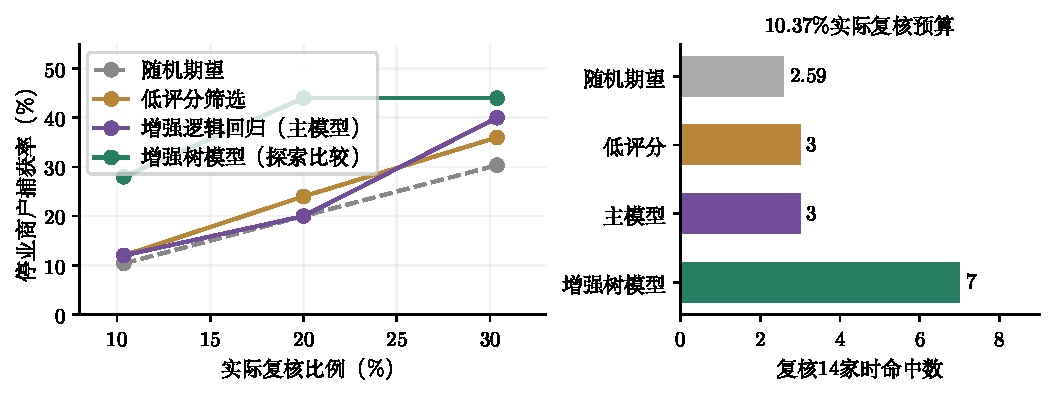
\includegraphics[width=1\linewidth]{figures/figure04_budget.pdf}
\caption{图4 不同复核预算下的停业商户捕获率及约10\%预算的命中数}
\end{figure}
\begin{table}[H]
\centering
\caption{表5 复核14家测试商户的模拟效果}
\setlength{\tablewidth}{\linewidth}
\addtolength{\tablewidth}{-10\tabcolsep}
\begin{tabular}{>{\raggedright\arraybackslash}p{0.350\tablewidth}>{\raggedright\arraybackslash}p{0.140\tablewidth}>{\raggedright\arraybackslash}p{0.190\tablewidth}>{\raggedright\arraybackslash}p{0.190\tablewidth}>{\raggedright\arraybackslash}p{0.130\tablewidth}}
\toprule
\textbf{策略} & \textbf{命中数} & \textbf{名单命中率} & \textbf{停业捕获率} & \textbf{提升倍数} \\
\midrule
随机抽查（期望） & 2.59 & 18.52\% & 10.37\% & 1.00 \\
低评分筛选 & 3 & 21.43\% & 12.00\% & 1.16 \\
质量基线LR·Q & 3 & 21.43\% & 12.00\% & 1.16 \\
主模型LR·QAT & 3 & 21.43\% & 12.00\% & 1.16 \\
增强树模型HGB·QAT & 7 & 50.00\% & 28.00\% & 2.70 \\
\bottomrule
\end{tabular}
\end{table}
随机名单2.59家为理论期望，不是某次抽查实际命中了小数家。主模型与低评分名单均命中3家，未表现出额外复核效率。增强树模型命中7家，提升倍数点估计为2.70，但95\%区间为[0.96，3.75]，包含1；模型相对随机的优势仍需独立复验。此树模型属于预设探索比较，不能因测试表现高而追认为已定型的部署模型。

增强树模型在约10\%预算下仍漏掉72\%的停止营业商户，且名单中一半商户仍在营业。因此这类输出更适合安排低成本人工核实，而非直接拒贷。该模拟也没有衡量真实违约、回收损失、核查成本或干预效果，不能将点估计转化为确定的商业收益。


\newpage
\section*{七、偏差检查、敏感性与研究限制}
营业与停止营业组的最后评论年份存在明显差异：551家营业商户中528家最后评论在2017年，123家停止营业商户中只有6家在2017年。图5展示这一结构与固定预测的追加日期审计。虽未输入年份，窗口年代仍可能影响评论量和消费行为；排除直接日期变量不能保证已消除混杂。

\begin{figure}[H]
\centering
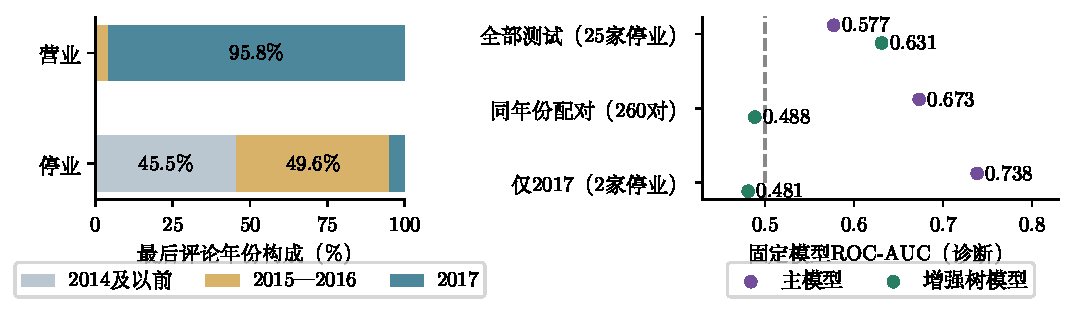
\includegraphics[width=1\linewidth]{figures/figure05_bias.pdf}
\caption{图5 日期结构及追加同年份审计（事后诊断，未重新拟合）}
\end{figure}
只比较同一年内停业—营业配对，共260对，主模型AUC为0.673，增强树为0.488；仅2017年107家（停业2家）时分别为0.738、0.481。树模型总体优势未在日期限制下保留，主模型较高子组分数也因事件极少而不稳定。该审计在原结果之后设计，未调参，不能作为确认性证据。原2015年及之后子样本主模型AUC仅0.525，仍需独立复验。

标签边界：没有关闭日期、统一状态采集日期、贷款逾期或真实流水，无法验证评论在风险事件之前可用。随机商户划分只检验同类历史记录的状态识别，不代表跨时间预警能力。停业也不能直接作为违约标签。

样本边界：平台消费者并非全部客群，评价数不等于营业额。新店、低评价量和长期无评论主体被排除；企业规模、连锁关系和评论真实性尚未核验。词典主题只反映低分评论中的话题提及，不是精确投诉归因。

外推与使用边界：评论截至2017年，海外区域样本不能证明2026年深圳小微企业适用性。当前官方数据协议及该镜像的再分发授权尚待核实，2015年历史协议[3]不能代替当前许可。本报告不披露原始评论及具名商户，正式提交前应确认教育比赛使用范围。


\newpage
\section*{八、产品思路与商业应用}
产品定位为“小微商户经营线索助手”，向银行客户经理输出“调查优先级＋触发指标＋可信度”。无足够评论时显示信息不足；有线索时核实经营和实际流水。画像可上线为信息展示，模型排序暂不进入自动授信。指标异常仅作核查理由，不当作真实经营问题的确证。

\begin{table}[H]
\centering
\caption{表6 产品闭环：从线索到可验证行动}
\setlength{\tablewidth}{\linewidth}
\addtolength{\tablewidth}{-6\tabcolsep}
\begin{tabular}{>{\raggedright\arraybackslash}p{0.220\tablewidth}>{\raggedright\arraybackslash}p{0.350\tablewidth}>{\raggedright\arraybackslash}p{0.430\tablewidth}}
\toprule
\textbf{模块} & \textbf{输出} & \textbf{建议动作} \\
\midrule
数据可用性 & 评论数量、覆盖跨度、更新情况 & 不足时提示“信息不足”，补充资料 \\
经营画像 & 评分变化、活跃度、低分主题 & 核实具体经营问题，查看实际流水 \\
调查排序 & 预算对应的待复核名单及原因 & 人工确认营业情况，记录误报与漏报 \\
反馈与验证 & 真实调查结果、成本与后续表现 & 定期复验，检验增量及商业价值 \\
\bottomrule
\end{tabular}
\end{table}
商业评价以每期复核k家为单位：净价值=k×(p×v-c)-F，其中p为前瞻验证的可行动风险命中率，v为每次有效发现的净收益，c为单家核查成本，F为期间固定成本。相对同预算低评分名单，增量价值=(命中差)×v-新增固定成本。本次主模型命中差为0，树模型为4，但停业命中不能代替可行动风险，不能据此估算节省金额。

\section*{九、总结结论}
第一，公开评论可以构建三维12项可解释的经营画像，便于在信息稀疏条件下形成调查线索。第二，本次主分析方案没有显示稳定的增量识别价值；增强树模型的探索性点估计较好，但模型差异和复核提升区间仍包含无改善，不能据此证明已具备金融风控能力。第三，日期混杂、标签缺失和历史地域限制决定了研究更适合可行性检验，尚不能支持自动授信或前瞻预警。

下一阶段采用统一月末观察点和之后90天经营核实标签；真实逾期单独验证。预先锁定流水基线、流水＋公开指标、10\%复核预算及成本口径，保留后续月份与新地区测试。试点保留随机抽查组，复核人员先独立确认再查看模型原因。仅在增量置信区间下界>0且净价值>0时扩大使用，否则维持画像展示和人工调查。此为待执行方案，不是已完成实验。


\newpage
\fancyfoot[C]{\fontsize{9pt}{12pt}\selectfont 参考文献}
\section*{参考文献与数据来源}
[1] Yelp. Yelp Open Dataset[EB/OL]. \url{https://www.yelp.com/dataset}. 官方当前使用条款在本次研究中尚未核实。

[2] Cleveland区域公开子集及筛选说明[DS/OL]. \url{https://github.com/ahegel/yelp-dataset}. 本研究固定提交e5b82be3c909f9bb45dfd03e164ae0b7897832bd；评论截至2017年7月26日，营业状态采集时间未说明。

[3] Yelp. Dataset Challenge Academic Dataset Terms of Use[EB/OL]. 更新日期2015-03-23. 历史协议归档来源：\url{https://github.com/vc1492a/Yelp-Challenge-Dataset}. 固定提交0402872665e57c253ba7dcbb71b10842bc1ef08a；文件位于该仓库Raw Data目录，题名为Dataset Challenge Academic Dataset Agreement。该历史归档不证明当前授权。

[4] scikit-learn. Model evaluation: quantifying the quality of predictions; LogisticRegression; HistGradientBoostingClassifier[EB/OL]. \url{https://scikit-learn.org/stable/}. 本研究AP采用average\_precision\_score的非插值平均精确率定义。

[5] Efron B, Tibshirani R J. An Introduction to the Bootstrap[M]. New York: Chapman \& Hall, 1993.

[6] Holm S. A Simple Sequentially Rejective Multiple Test Procedure[J]. Scandinavian Journal of Statistics, 1979, 6(2): 65–70.


\end{document}
